% Autor: Leonhard Segger, Alexander Neuwirth
% Datum: 2017-10-30
\documentclass[
	% Papierformat
	a4paper,
	% Schriftgröße (beliebige Größen mit „fontsize=Xpt“)
	12pt,
	% Schreibt die Papiergröße korrekt ins Ausgabedokument
	pagesize,
	% Sprache für z.B. Babel
	ngerman
]{scrartcl}

% Achtung: Die Reihenfolge der Pakete kann (leider) wichtig sein!
% Insbesondere sollten (so wie hier) babel, fontenc und inputenc (in dieser
% Reihenfolge) als Erstes und hyperref und cleveref (Reihenfolge auch hier
% beachten) als Letztes geladen werden!

% Silbentrennung etc.; Sprache wird durch Option bei \documentclass festgelegt
\usepackage{babel}
% Verwendung der Zeichentabelle T1 (Sonderzeichen etc.)
\usepackage[T1]{fontenc}
% Legt die Zeichenkodierung der Eingabedatei fest, z.B. UTF-8
\usepackage[utf8]{inputenc}
% Schriftart
\usepackage{lmodern}
% Zusätzliche Sonderzeichen
\usepackage{textcomp}

% Mathepaket (intlimits: Grenzen über/unter Integralzeichen)
\usepackage[intlimits]{amsmath}
% Ermöglicht die Nutzung von \SI{Zahl}{Einheit} u.a.
\usepackage{siunitx}
% Zum flexiblen Einbinden von Grafiken (\includegraphics)
\usepackage{graphicx}
% Abbildungen im Fließtext
\usepackage{wrapfig}
% Abbildungen nebeneinander (subfigure, subtable)
\usepackage{subcaption}
% Funktionen für Anführungszeichen
\usepackage{csquotes}
\MakeOuterQuote{"}
% Zitieren, Bibliographie
\usepackage{biblatex}


% Zur Darstellung von Webadressen
\usepackage{url}
%chemische Formeln
\usepackage[version=4]{mhchem}
% siunitx: Deutsche Ausgabe, Messfehler getrennt mit ± ausgeben
\usepackage{floatrow}
\floatsetup[table]{capposition=top}
\usepackage{float}
% Verlinkt Textstellen im PDF-Dokument
\usepackage[unicode]{hyperref}
% "Schlaue" Referenzen (nach hyperref laden!)
\usepackage{cleveref}
\sisetup{
	locale=DE,
	separate-uncertainty
}
%\bibliography{14Mo_O2_11-06-2018_References}

\begin{document}
	
	\begin{titlepage}
		\centering
		{\scshape\LARGE Versuchsbericht zu \par}
		\vspace{1cm}
		{\scshape\huge O2 - Mikrowellen \par}
		\vspace{2.5cm}
		{\LARGE Gruppe 14Mo \par}
		\vspace{0.5cm}
		
		{\large Alexander Neuwirth (E-Mail: a\_neuw01@wwu.de) \par}
		{\large Leonhard Segger (E-Mail: l\_segg03@uni-muenster.de) \par}
		\vfill
		
		durchgeführt am 11.06.2018\par
		betreut von\par
		{\large Stephan Majert}
		
		\vfill
		
		{\large \today\par}
	\end{titlepage}
	\tableofcontents
	\newpage

	%TODO mehr TODO in Default	

	\section{Kurzfassung}
	%TODO Hypothese	und deren Ergebnis, wenn Hypothese ist, dass nur Theorie erfüllt, sagen: Erwartung: Theorie aus einführung (mit reflink) erfüllt
	%TODO Ergebnisse, auch Zahlen, mindestens wenn's halbwegs Sinn ergibt
	%TODO Was wurde gemacht
	%TODO manche leute wollen Passiv oder "man", manche nicht
	
	%TODO Vgl. Bestrahlung beide Seiten Halbzylinder Hyp
	\section{Methoden}
	%TODO Bilder von der Website klauen
	%TODO Polarisationscheck ?
	Es wird der Mikrowellensender auf einer Schiene und der Empfänger auf  einer sich dazu senkrecht befindenden befestigt.
	Dann wird durch Drehung des Senders um die Strahlungsachse die Polarisationsebene geändert, bis die vom Empfänger gemessene Intensität maximal ist. %TODO ist das mit der Achse klar?
	Die Intensität am Empfänger wird für unterschiedliche Abstände des Empfängers von der Strahlungsachse gemessen.
	Dies wird für unterschiedliche Abstände des Senders zur orthogonalen Schiene des Empfängers durchgeführt, um den virtuellen Quellfleck des Senders bestimmen zu können.
	
	Dann wird eine Metallplatte in den Strahlengang gebracht, sodass sie die Strahlung reflektieren und eine stehende Welle bilden kann.
	Während mit einem Empfänger nach den Knoten gesucht wird, wird der Abstand der Metallplatte zur Quelle optimiert, bis die Knote möglichst gut ausgebildet sind. %klar?
	Die Positionen mehrerer Knoten wird gemessen, um daraus die Wellenlänge bestimmen zu können. %TODO sollte man so Sinn angeben?
	
	Ein PVC-Halbzylinder wird anstelle der Platte in den Strahlengang gebracht.
	Dieser ist drehbar gelagert, sodass der Einfallwinkel variabel ist.
	Für mehrere Einfallwinkel wird mit einem Empfänger der Winkel der maximalen Transmission gesucht und gemessen.
	Dies wird zweimal durchgeführt.
	Dabei wird einmal der Halbzylinder so gedreht, dass die Welle erst durch die flache Seite des Halbzylinders und dann die runde fällt und einmal so, dass es andersherum stattfindet.
	
	Dann wird der Halbzylinder so gedreht, dass an der flachen Seite Totalreflexion zu beobachten ist. %TODO ist dass zu unpräzise?
	Ein zweiter Halbzylinder wird auf die Transmissionsseite des ersten gebracht und die Intensität der Strahlung hinter dem zweiten Halbzylinder in Abhängigkeit vom Abstand der beiden Zylinder gemessen.
	
	Zuletzt wird ein Schaumstoffquader, in dem sich ein dreidimensionales Gitter aus Metallkugeln befindet, in den Strahlengang gebracht und bei variablem Einfallswinkel die Intensität am gleich groß gewählten Reflexionswinkel gemessen.
	\begin{figure}[H] 
		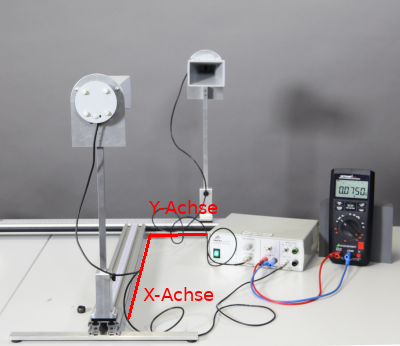
\includegraphics[width=0.7\textwidth]{MikrowellenMitAchsen}
		\centering
		\caption{Aufbau zur Bestimmung des Quellflecks mit den jeweiligen Achsenbeschriftungen.}
		\label{fig_mikrowellenmitachsen}
		\centering
	\end{figure}
	\section{Ergebnisse und Diskussion}
	%TODO Unsicherheiten
	

	%TODO Einflüsse von veränderten Parametern auf Messung
	\subsection{Beobachtungen und Datenanalyse}
	\subsubsection{Unsicherheiten} %TODO GGF IN DATENANYLSY
	Die Unsicherheiten wurden gemäß GUM ermittelt. 
	Außerdem wurde für Unsicherheitsrechnungen die Python Bibliothek "uncertainties" verwendet.
	\begin{description}
		\item[Messleiste:] Die Unsicherheit der Messleiste wurde auf \SI{0,2}{cm} abgeschätzt (dreieckige WDF).
		\item[Maßband/Geodreieck:] Die Unsicherheit des Maßbands/Geodreiecks wurde mit \SI{0,05}{cm} bemessen (dreieckige WDF).
		\item[Winkelmessung:]  Die Winkel wurden mit dem Auge anhand einer Skala abgelesen, wobei die Unsicherheit \SI{0,4}{\degree} beträgt. Beim Verstellen des Winkelmessarmes hat dieser jedoch viel Spielraum gehabt in dem sich der Winkelzeiger nicht verändert hat. Deshalb wurde für diese Messung die doppelte Unsicherheit gewählt.
		\item[Multimeter:] Das Multimeter zeigte die Spannung mit 2 Nachkommastellen an. Da bei den Messungen die Anzeige der letzten Ziffer schwankte, wurde die Unsicherheit mit \SI{0,03}{V} abgeschätzt (rechteckige WDF).
	\end{description}

	\subsubsection{Bestimmung des Quellflecks des Senders}
	Es wurde in vier verschiedenen Abständen zum Sender orthogonal 11 Intensitäten gemessen die Strahlung gemessen.
	Die gemessenen Strahlenprofile sind in \crefrange{fig_74cm}{fig_114cm} dargestellt. 
	\begin{figure}[H] %TODO X-Achsen-Abstand ist kein schöner Ausdruck.
		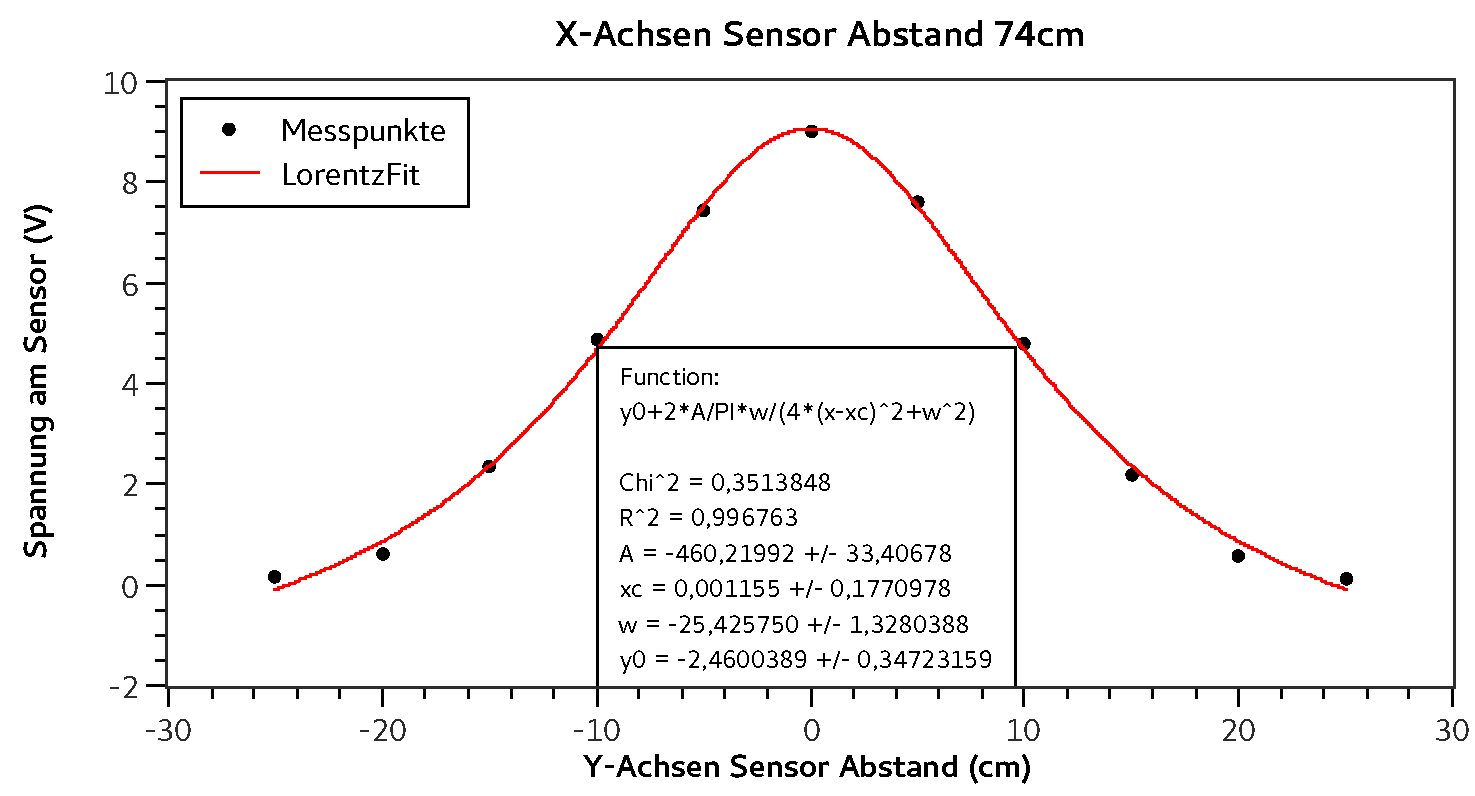
\includegraphics[width=1\textwidth]{fig_74cm}
		\centering
		\caption{Strahlenprofil im Abstand von \SI{74}{cm}. Die Unsicherheiten sind kleiner als die Symbolgröße.}
		\label{fig_74cm}
		\centering
	\end{figure}

	\begin{figure}[H]
		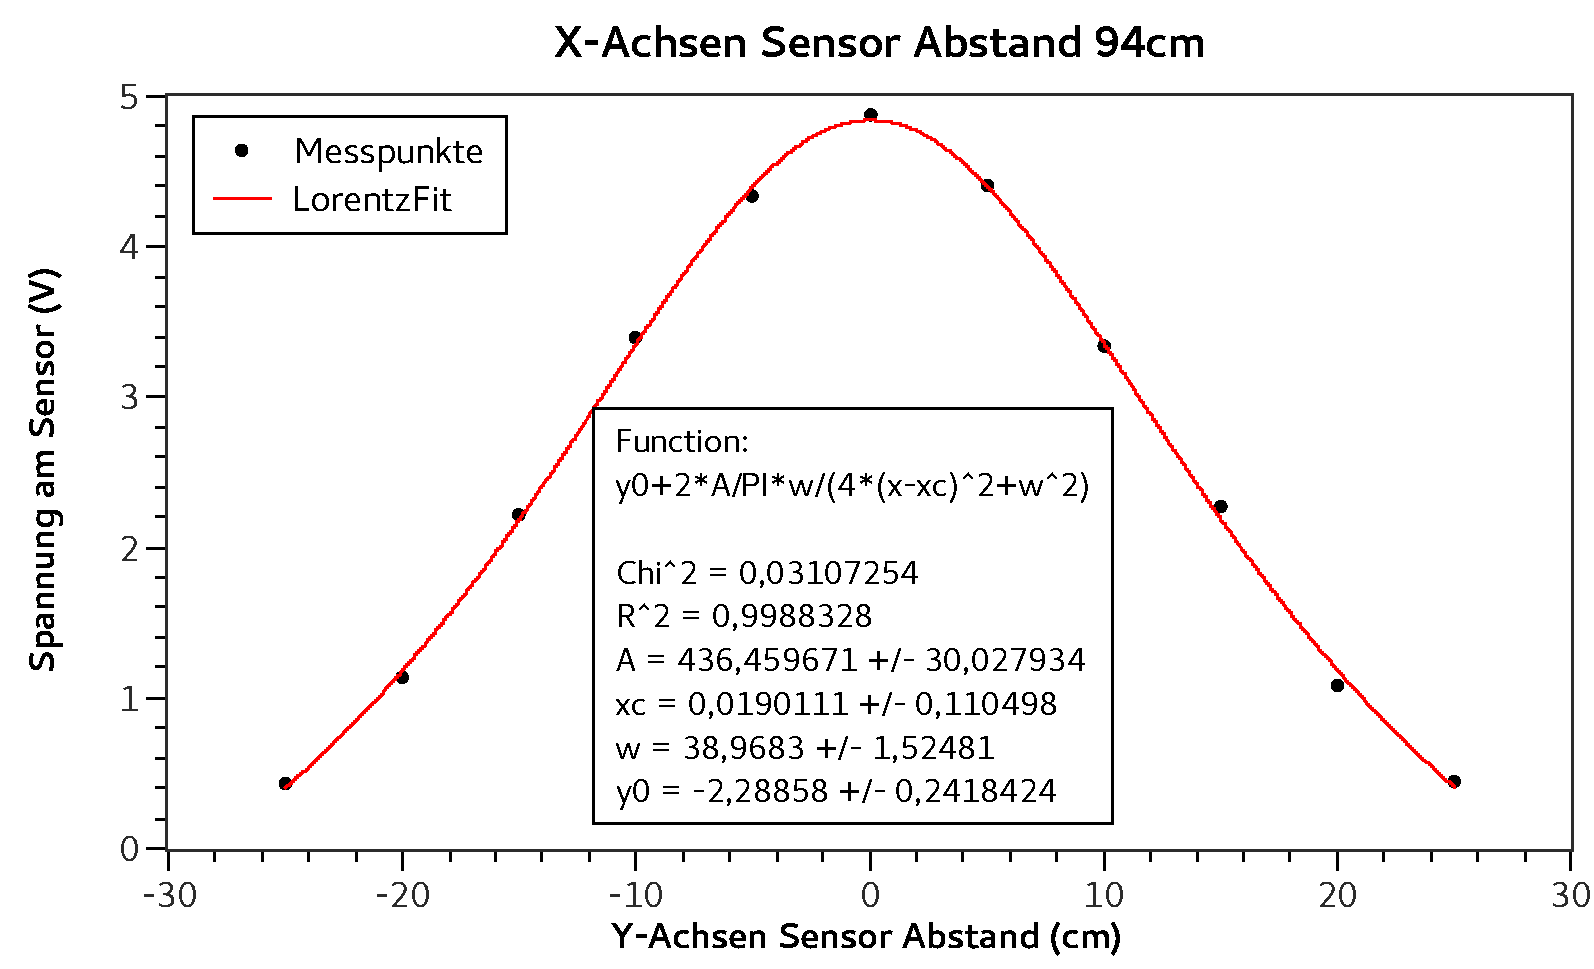
\includegraphics[width=1\textwidth]{fig_94cm}
		\centering
		\caption{Strahlenprofil im Abstand von \SI{94}{cm}. Die Unsicherheiten sind kleiner als die Symbolgröße.}
		\label{fig_94cm}
		\centering
	\end{figure}
	\begin{figure}[H]
		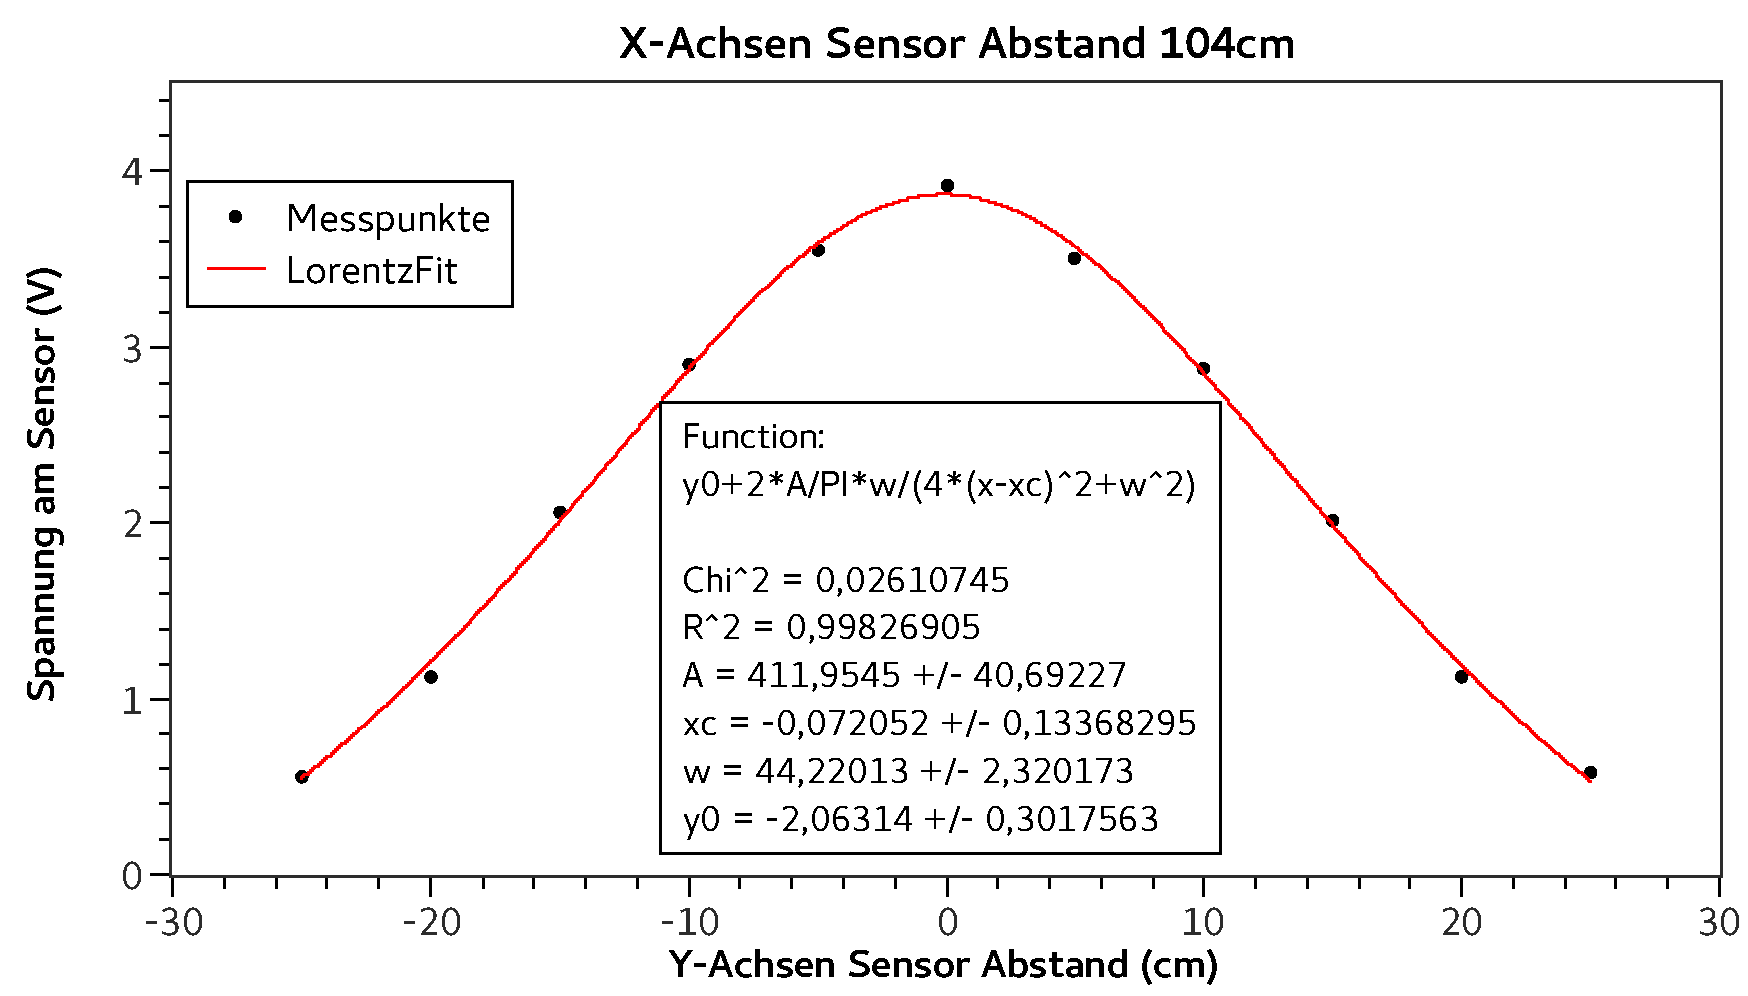
\includegraphics[width=1\textwidth]{fig_104cm}
		\centering
		\caption{Strahlenprofil im Abstand von \SI{104}{cm}. Die Unsicherheiten sind kleiner als die Symbolgröße.}
		\label{fig_104cm}
		\centering
	\end{figure}
	\begin{figure}[H]
		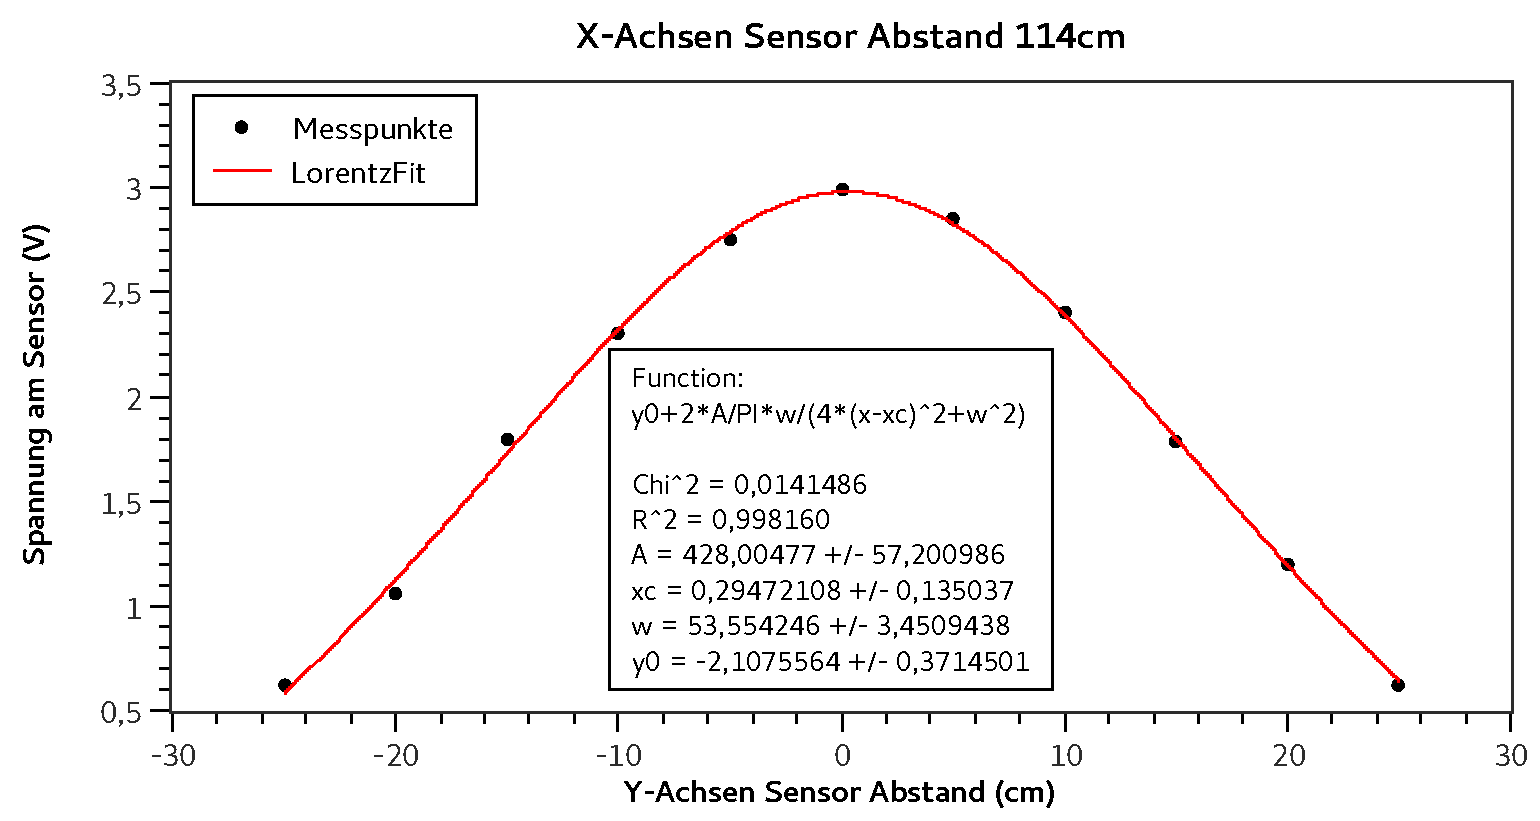
\includegraphics[width=1\textwidth]{fig_114cm}
		\centering
		\caption{Strahlenprofil im Abstand von \SI{114}{cm}. Die Unsicherheiten sind kleiner als die Symbolgröße.}
		\label{fig_114cm}
		\centering
	\end{figure}
	Um die Abweichung des Quellflecks des Senders zu dessen Position zu bestimmen, wurde ein Lorentzkurven-Fit durchgeführt. Die resultierenden $xc$ in den Graphen sind in \cref{tab_xc} aufgeführt:
	\begin{table}[H]
		\centering
		\begin{tabular}{ c | c }
			Abstand Sender/Empfänger in \SI{}{cm} & $xc$ in \SI{}{cm}  \\ \hline
			\SI{74}{}&\SI{0,00+-0,17}{}\\
			\SI{94}{}&\SI{0,02+-0,11}{}\\
			\SI{104}{}&\SI{0,07+-0,13}{}\\
			\SI{114}{}&\SI{0,29+-0,13}{}\\
		\end{tabular}
		\caption{Zur Strahlungsrichtung orthogonale Abweichung $xc$ des Quellpunkts zum Sender.}
		\label{tab_xc} 
	\end{table}
	Unter der Annahme, dass die Strahlung in der Tischebene als Kugelwelle genähert werden kann, nimmt die Intensität mit $1/r^2$ ab. 
	Deshalb wurde in \cref{fig_y0cm} die Fitfunktion $f(x)=a*(1/(x+b)^2)$ berechnet. 
	$b=\SI{-20,55+-1,95}{cm}$ ist die Verschiebung des Quellflecks zur Position des Senders, d.h. der Quellfleck befindet sich vor dem Sender. %TODO Das finde ich recht überraschend. - Ich hingegen hatte keine Erwartungen.
	\begin{figure}[H]
		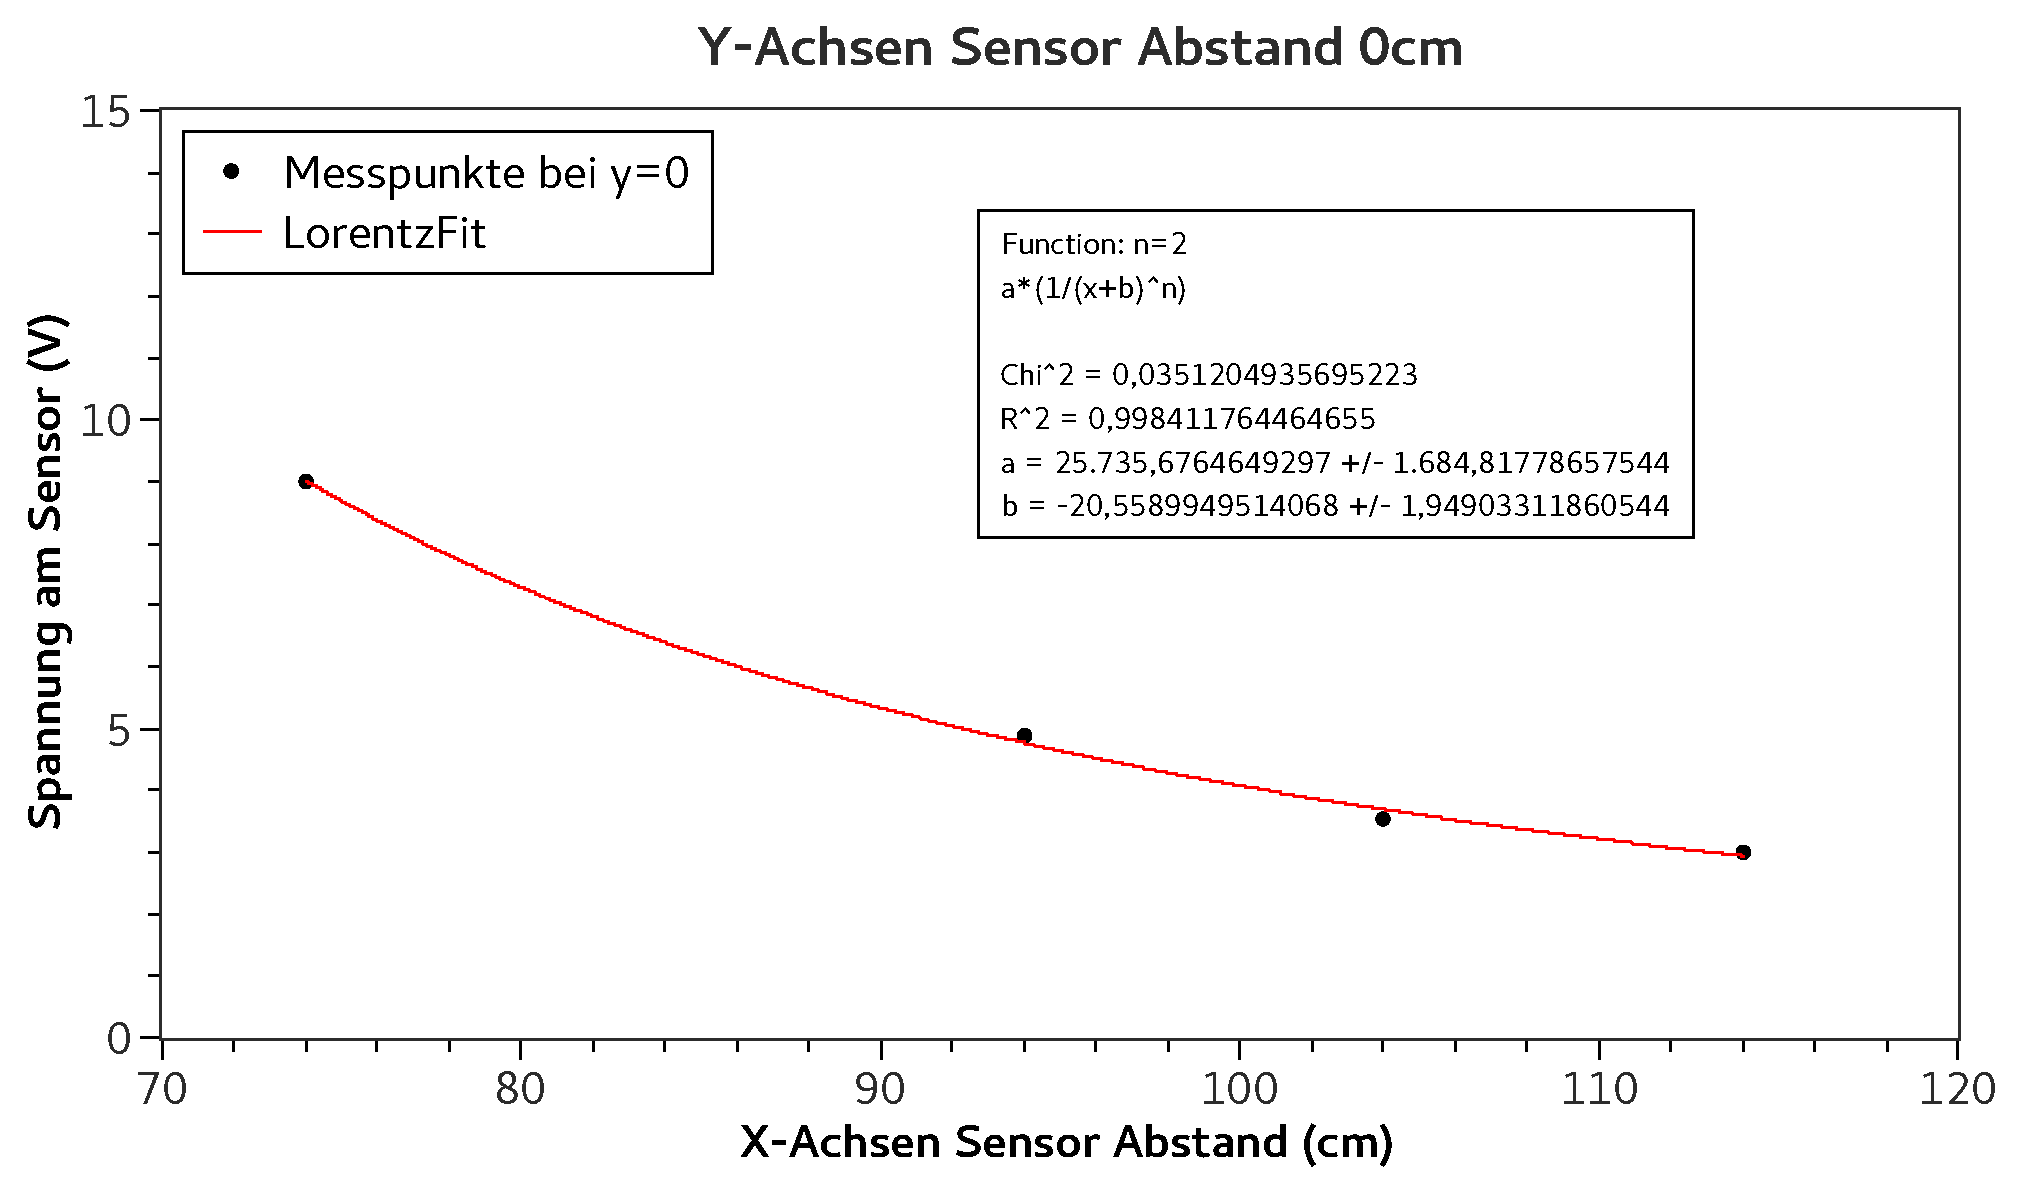
\includegraphics[width=1\textwidth]{fig_y0cm}
		\centering
		\caption{Die Maxima der Strahlenprofile sind gegen den Abstand des Sensors in X-Richtung aufgetragen. Die Unsicherheiten sind kleiner als die Symbolgröße.}
		\label{fig_y0cm}
		\centering
	\end{figure}
	%TODO Wie aussagekräftig ist das, weil der "Empfangsfleck" ja auch nicht bekannt ist? - Gibt es sowas überhaupt?
	
	\subsubsection{Bestimmung der Wellenlänge}
	Bei der bestmöglichen Auflösung der Knoten der stehenden Welle betrug die Spannung an den Minima (Knoten) noch \SI{0,03}{V}.
	In \cref{fig_steh_welle} sind die Positionen der Minima aufgelistet.
	Die gemessenen Positionen der jeweiligen Strahlungsminima wurden linear angeordnet. 
	Die gemittelte halbe Wellenlänge ergibt sich aus dem Abstand des ersten zum letzten Minimum geteilt durch die Anzahl der Minima. %Theoretisch wäre halt die einzelnen zu Mitteln möglicherweise präziser. - Nein, ich habe bsplw. auch nen Fit in den Graphen gemacht aber das ist halt ungenauer, weil er die Abstände zu den Punkten minimiert. Wenn man aber weiß, dass 10 Knoten drin sind, mitteln sich die einzelnen Abweichungen, wenn man nur die Grenzen anschaut gut weg. (Es konnte ja nicht ganz exakt der Knoten festgestellt werden
	So folgt: 
	\begin{equation}
		\lambda = 2 \cdot \frac{\SI{28,1 +- 0,2}{cm} + \SI{12,4+-0,2}{cm}}{10} = \SI{3,14 +- 0,05}{cm}.
	\end{equation}
	\begin{figure}[H] %TODO Die Punkte sind in der Grafik sehr schlecht zu erkennen.
		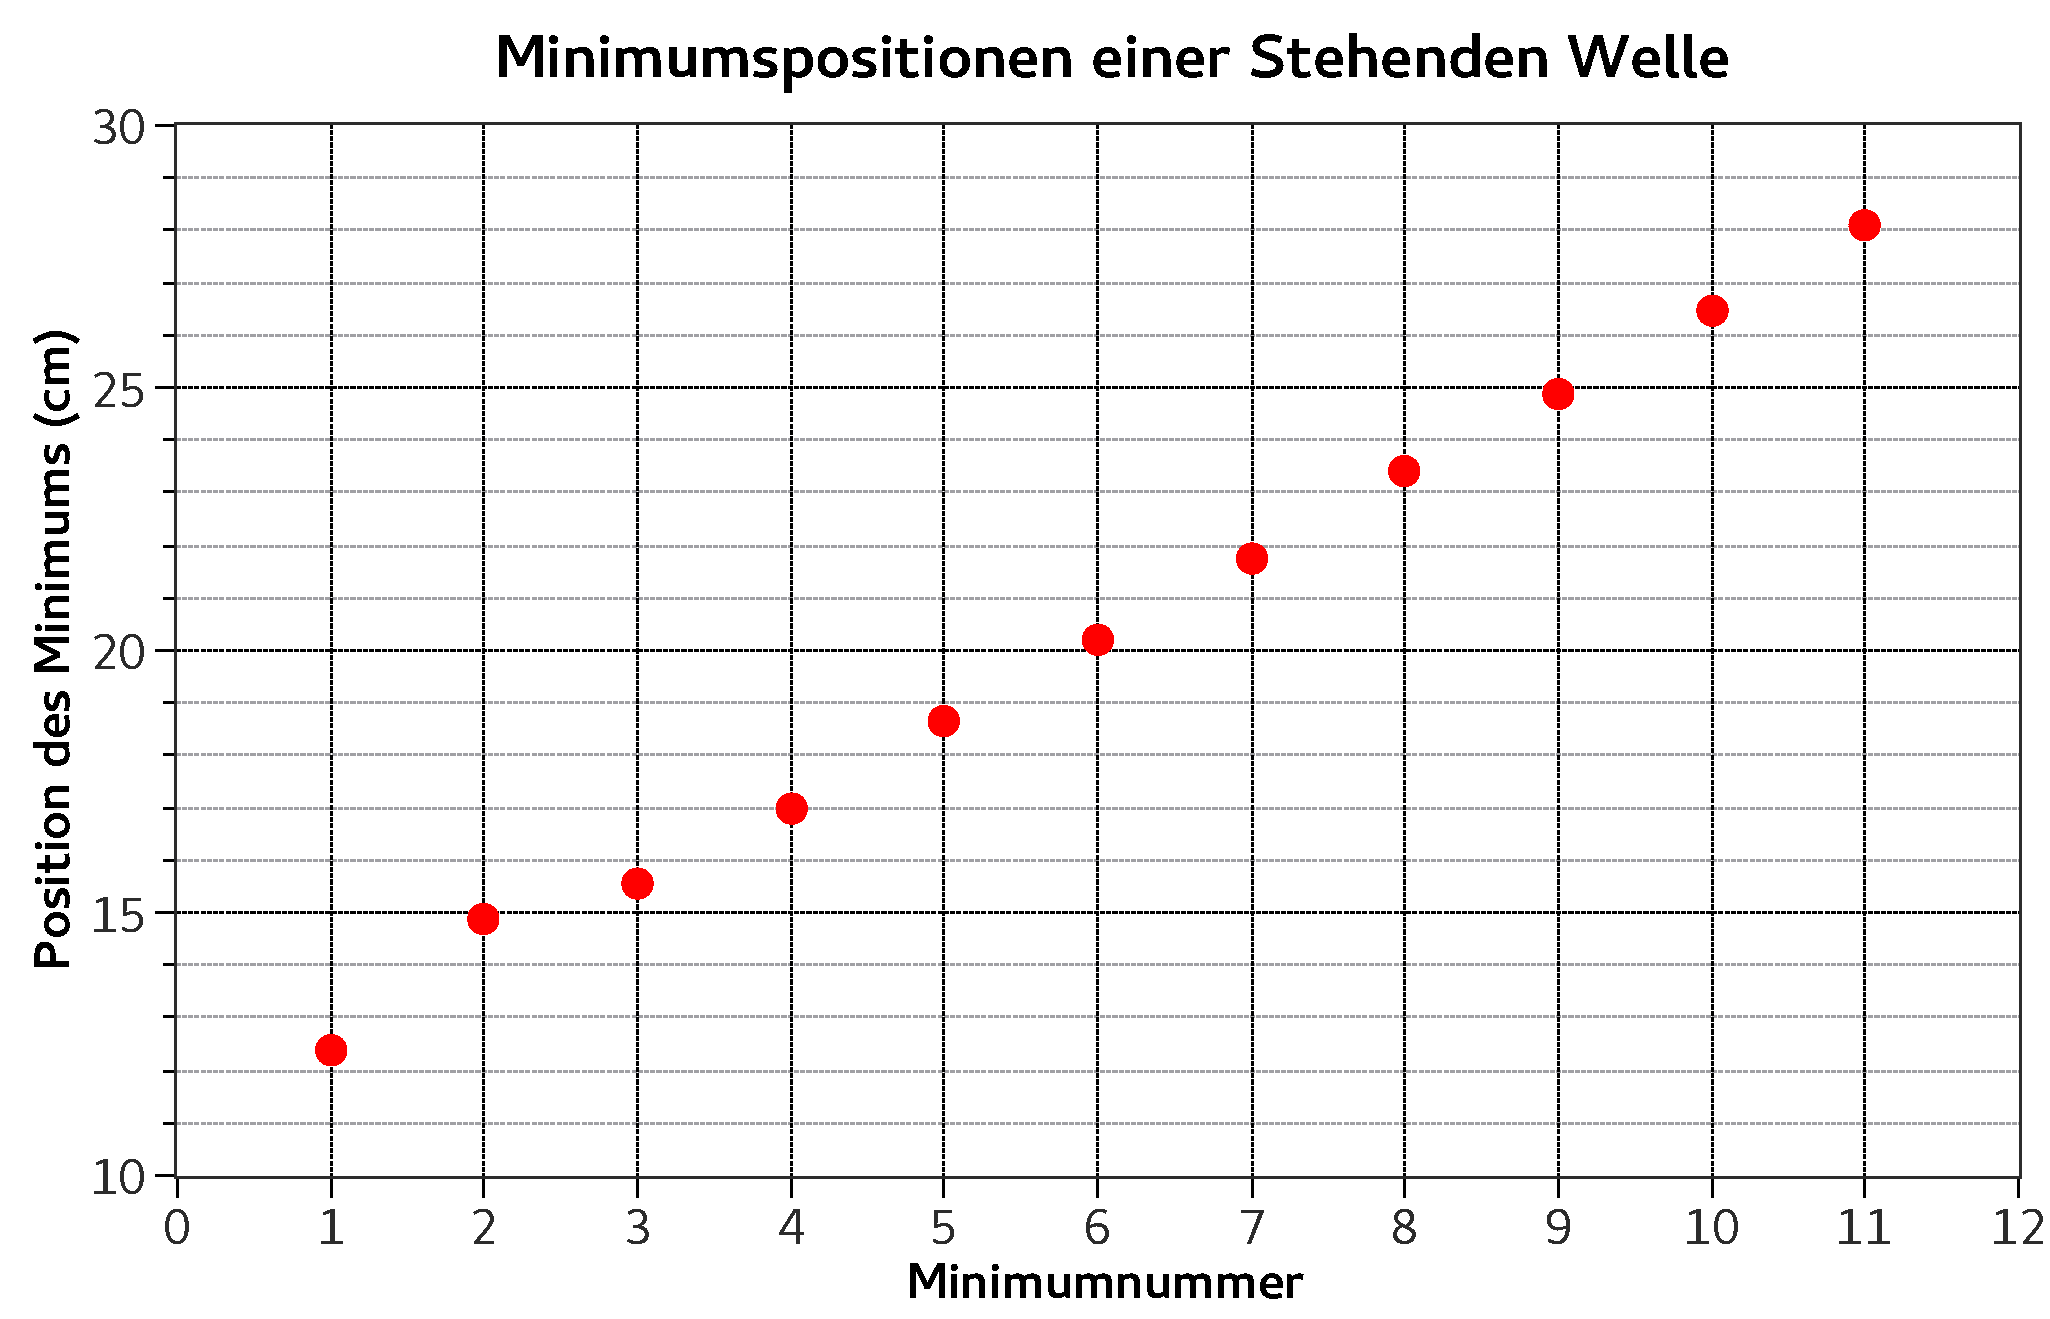
\includegraphics[width=0.7\textwidth]{fig_steh_welle}
		\centering
		\caption{Hier sind die gemessenen Positionen der Knoten der stehenden Welle dargestellt. Die Unsicherheiten sind kleiner als die Symbolgröße.}
		\label{fig_steh_welle}
		\centering
	\end{figure}
	\subsubsection{Bestimmung des Brechungsindex von PVC}
	Der Brechungsindex von PVC für Mikrowellen wurde auf zwei Arten bestimmt. 
	Zuerst wurde die runden Seite des Halbzylinders in verschiedenen Winkeln bestrahlt und der Winkel des Maximums der transmittierten Strahlung gemessen.
	Die Messergebnisse sind in \cref{fig_rund_zyl} aufgeführt.
	Das Snelliusschen Brechungsgesetzt lautet:
	\begin{equation}
		n_i \cdot \sin(\vartheta_i) = n_t \cdot \sin(\vartheta_t)
		\label{eq_snellius}
	\end{equation}
	Somit kann der Brechungsindex $n_\text{PVC}$  mit 
	\begin{equation}
		n_\text{PVC} = \frac{\sin(\beta)}{\sin(\alpha)} n_\text{Luft}
	\end{equation}
	bestimmt werden.
	Da $n_\text{Luft}$ ungefähr 1 ist, ist die Steigung des linearen Fits in \cref{fig_rund_zyl} gleich $n_\text{PVC}=\SI{1,56 +- 0,05}{}$.

	\begin{figure}[H]
		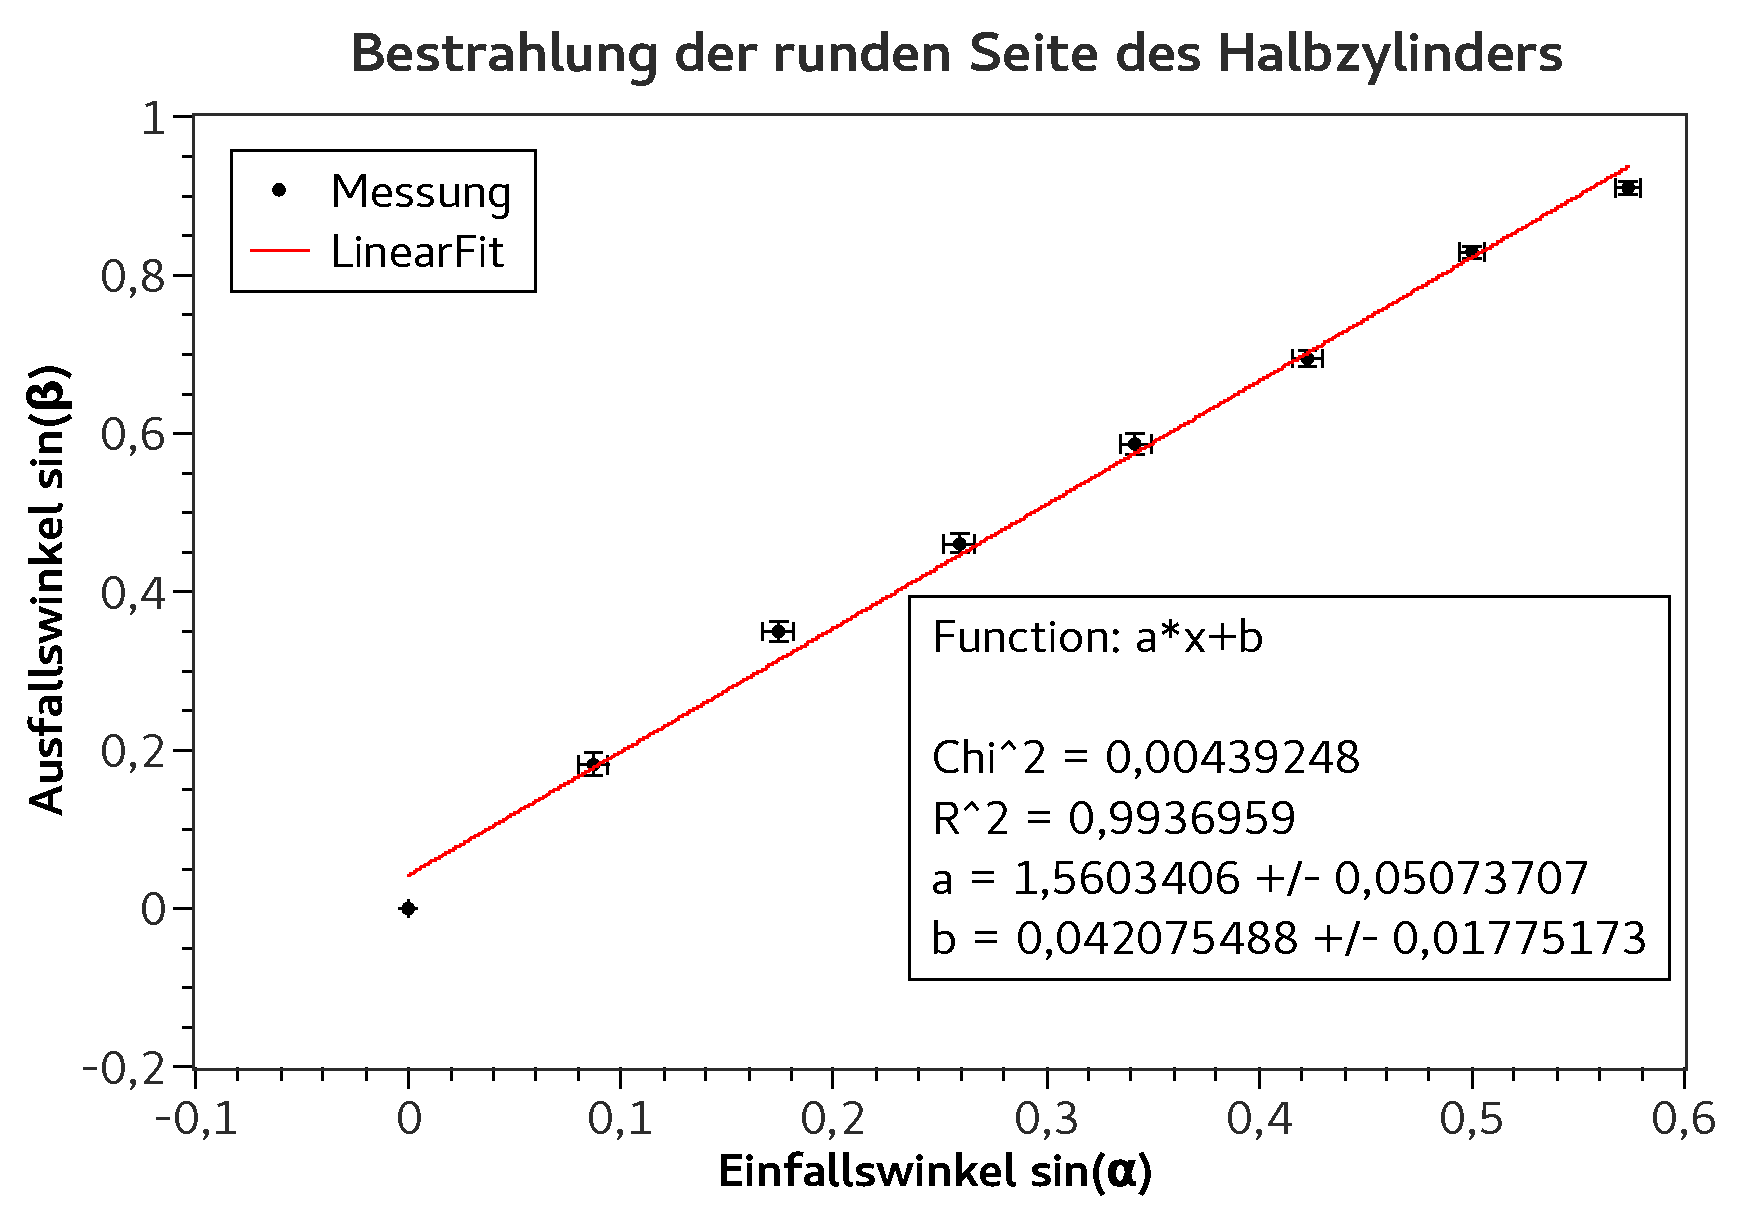
\includegraphics[width=0.7\textwidth]{fig_rund_zyl}
		\centering
		\caption{Der Sinus des Ausfallwinkels ist gegen den Sinus des Einfallwinkels beim Bestrahlen der runden Seite des Halbzylinders aus PVC aufgetragen.}
		\label{fig_rund_zyl}
		\centering
	\end{figure}

	Als zweite Messmethode wurde die flache Seite des Halbzylinders bestrahlt.
	Die Rechnung erfolgt analog zur vorherigen, jedoch ist das Verhältnis der Sinusse der Winkel invertiert.
	Das heißt, die Steigung ist der Kehrwert des Brechungsindex von PVC.
	Aus der Steigung $a$ in \cref{fig_flach_zyl} von \SI{0,634+-0,020}{} folgt $n_\text{PVC} = \SI{1,57 +- 0,05}{}$.
	\begin{figure}[H]
		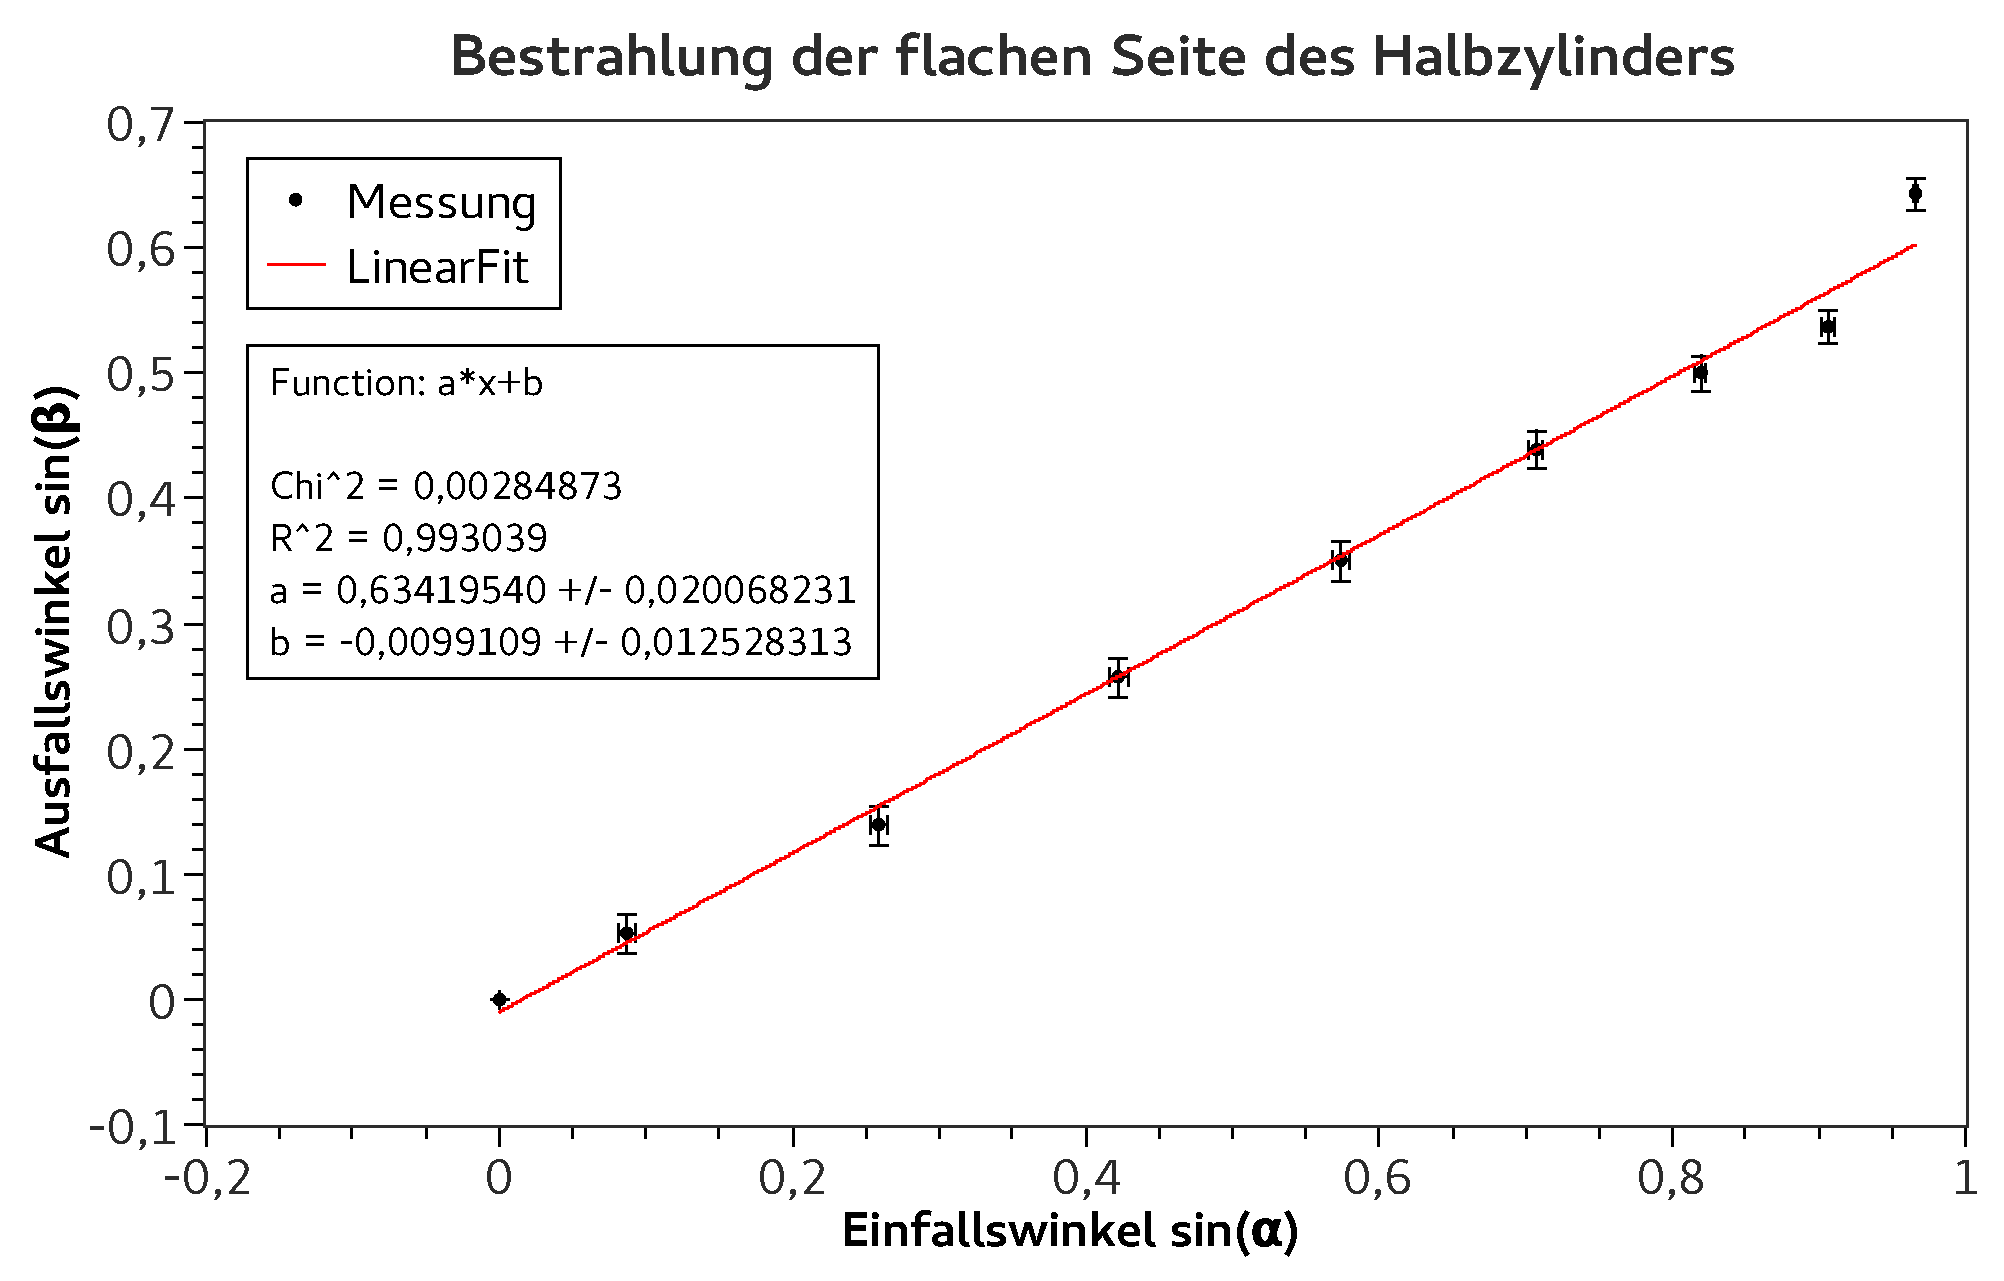
\includegraphics[width=0.7\textwidth]{fig_flach_zyl}
		\centering
		\caption{Der Sinus des Einfallwinkels $\alpha$ ist gegen den Sinus des Ausfallwinkels $\beta$, beim Bestrahlen der flachen Seite des Halbzylinders aus PVC, aufgetragen.}
		\label{fig_flach_zyl}
		\centering
	\end{figure}

	\subsubsection{Frustierte Totalreflexion}
	Es wurde die Intensität der transmittierten Strahlung als Funktion der Lückenbreite gemessen und in \cref{fig_frust_total} abgebildet.
	\begin{figure}[H] %TODO Man könnte was exponentielles reinfitten, weil man soll ja zeigen, dass es expo ist. - Hab ich jeztz (noch?!?) nicht gemacht, da man da ja nichts quantitativ rauszeihen soll, sondern mehr so diskutier/qualitativ
		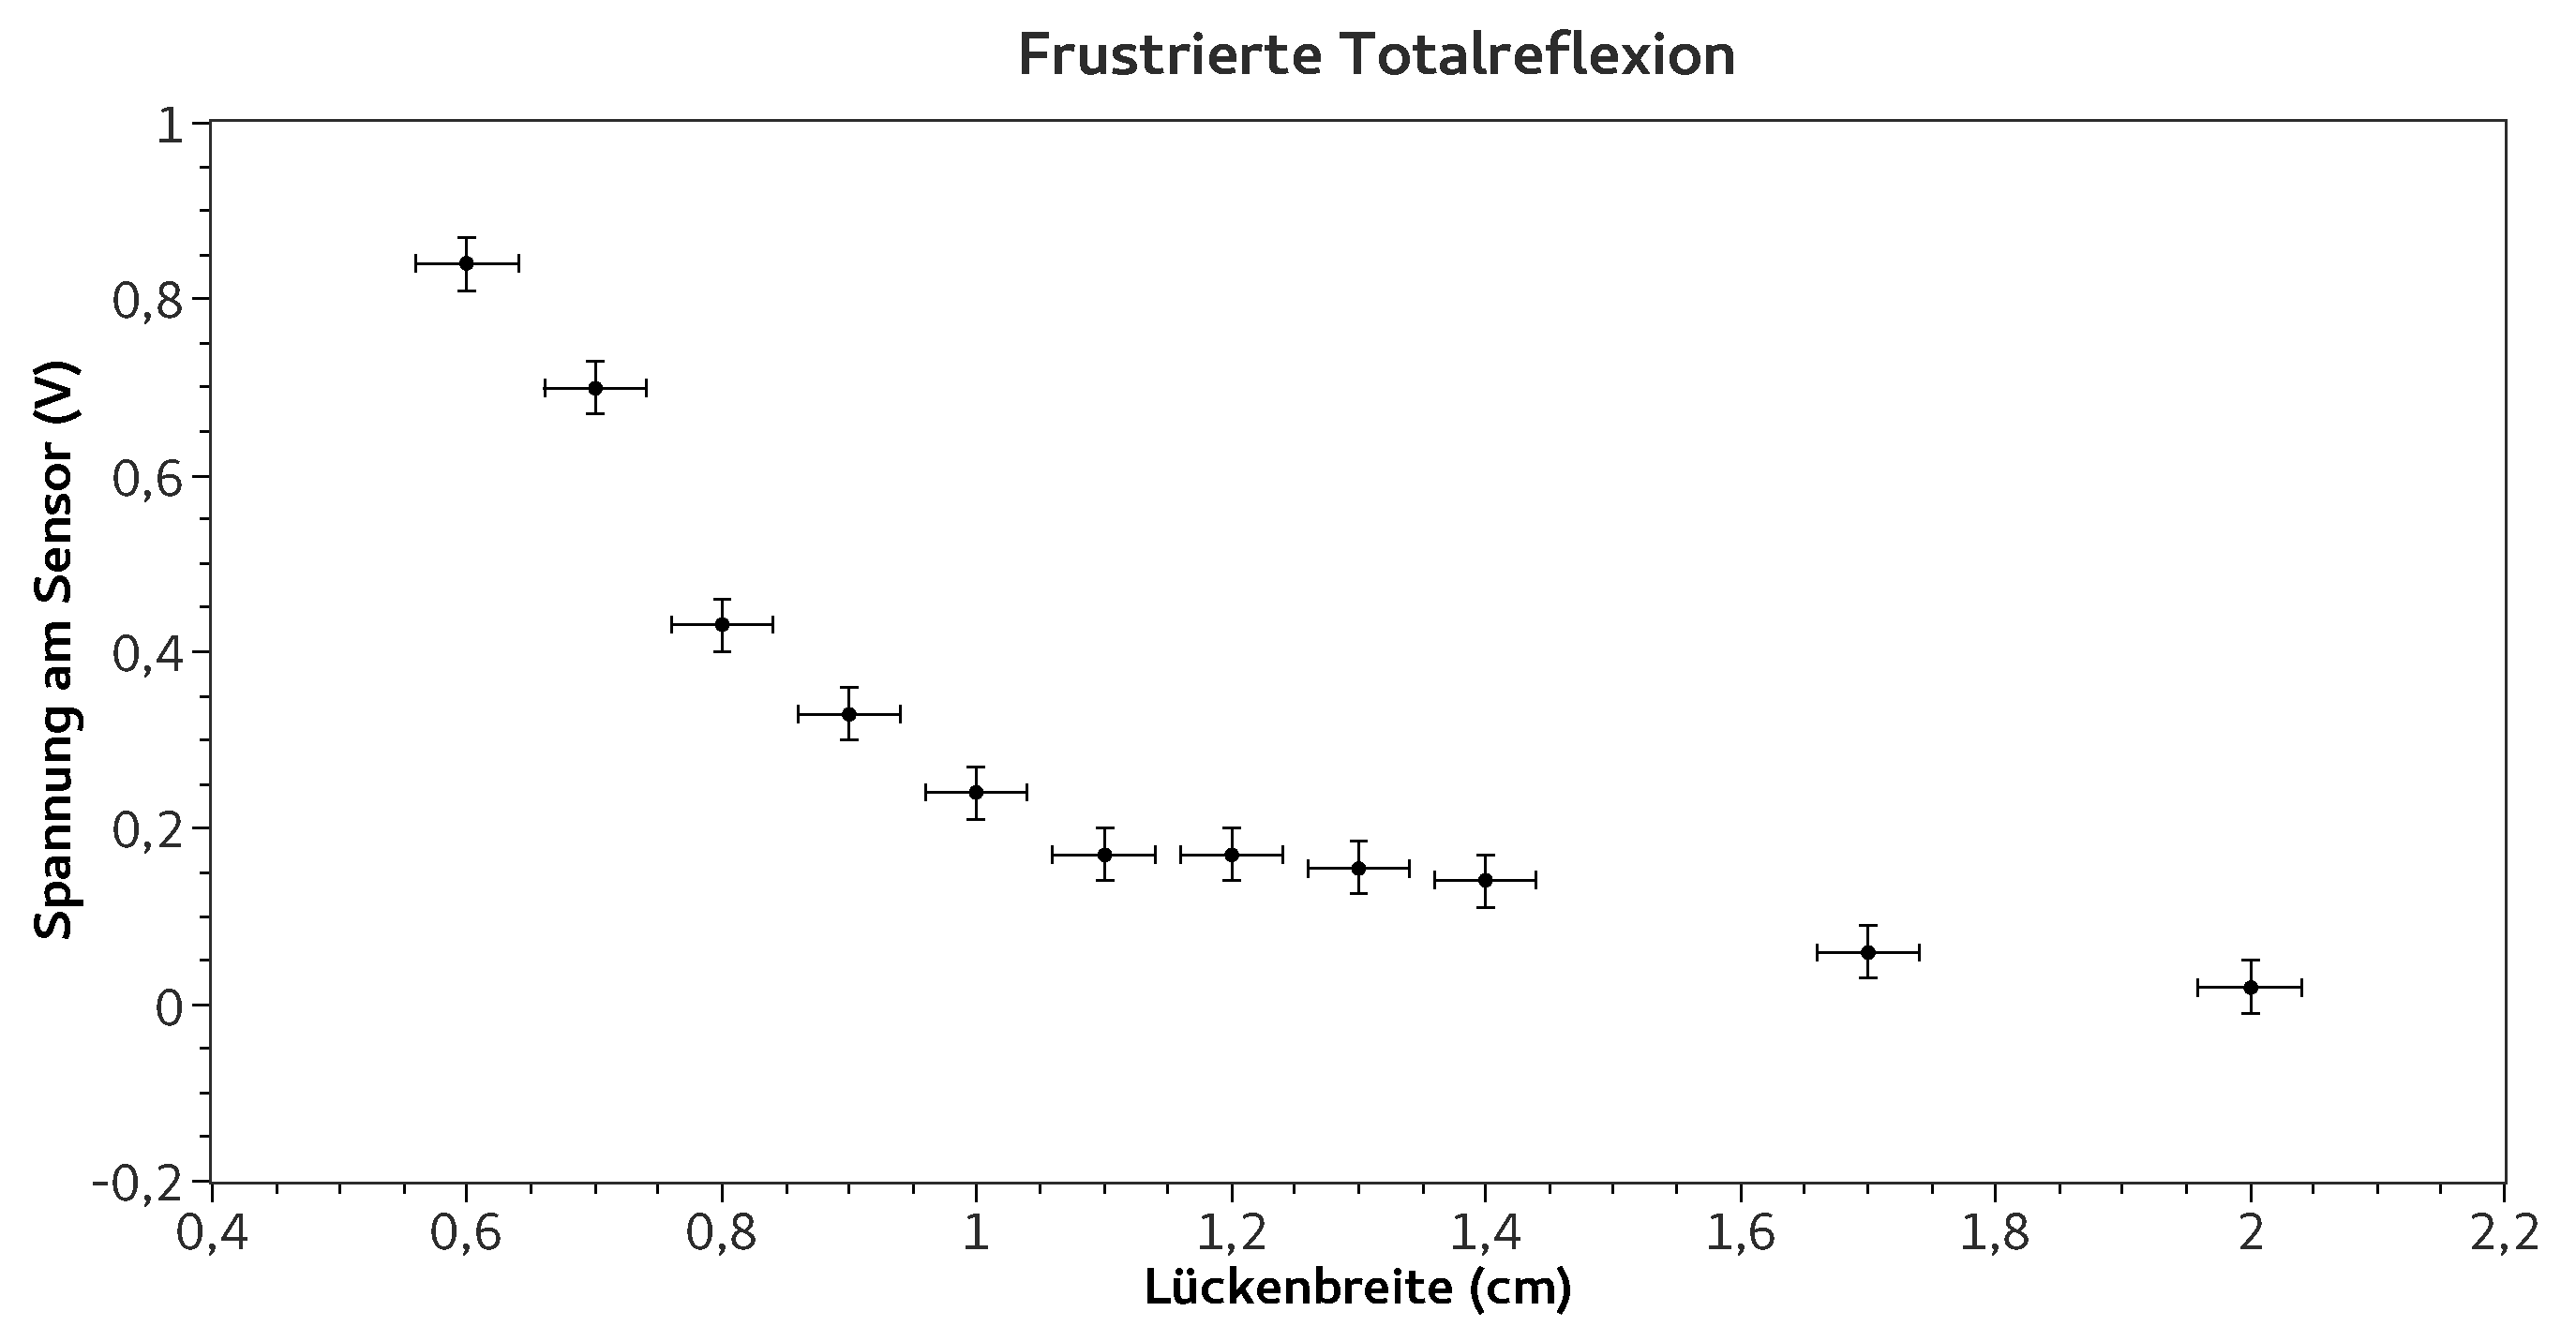
\includegraphics[width=0.7\textwidth]{fig_frust_total}
		\centering
		\caption{Gemessene Intensität der transmittierten Strahlung nach zwei Halbzylindern bei variiertem Lückenabstand.}
		\label{fig_frust_total}
		\centering
	\end{figure}

	\subsubsection{Bragg-Reflexion}
	Die Braggsche Reflexionsbedingung lautet:
	\begin{equation}
		2d \sin(\alpha) = n \lambda
	\end{equation}
	Wobei n = 1,2,... ist. %why no elem N - zu kompliziert, war so schneller, weil grad im Flow.
	In \cref{fig_bragg} wird die Reflexion bei einem Winkel von \SI{55,+-1}{\degree} maximal. %TODO warum ist die Unsicherheit nicht /sqrt(6) ? - Am Graph ist nur so abgeschätzt, da sind ja zwei Überlappende Unsicherheiten.
	Folglich ist 
	\begin{equation*}
		\frac{\lambda}{2sin(\alpha)} = \SI{1,93+-0,06}{cm}. %TODO War das so gemeint? - Man soll d bestimmen
	\end{equation*}
	Es kann nicht ausgeschlossen werden, dass für kleinere $\alpha$ ein Maximum vorhanden wäre.
	Deshalb ist eine Bestimmung der Gitterkonstante nicht möglich.
	Beim direkten Messen der Abstände der Kugeln im Schaumstoff ergab sich ein Abstand von \SI{3,875+-0,2}{cm}, woraus ersichtlich ist, dass das Maximum bei \SI{55}{\degree} dem bei $n=2$ entspricht. %TODO ohne Erklärung/Rechnung ist das nicht ersichtlich - 1,93*2 = 3,87 ?!?!?
	\begin{figure}[H]
		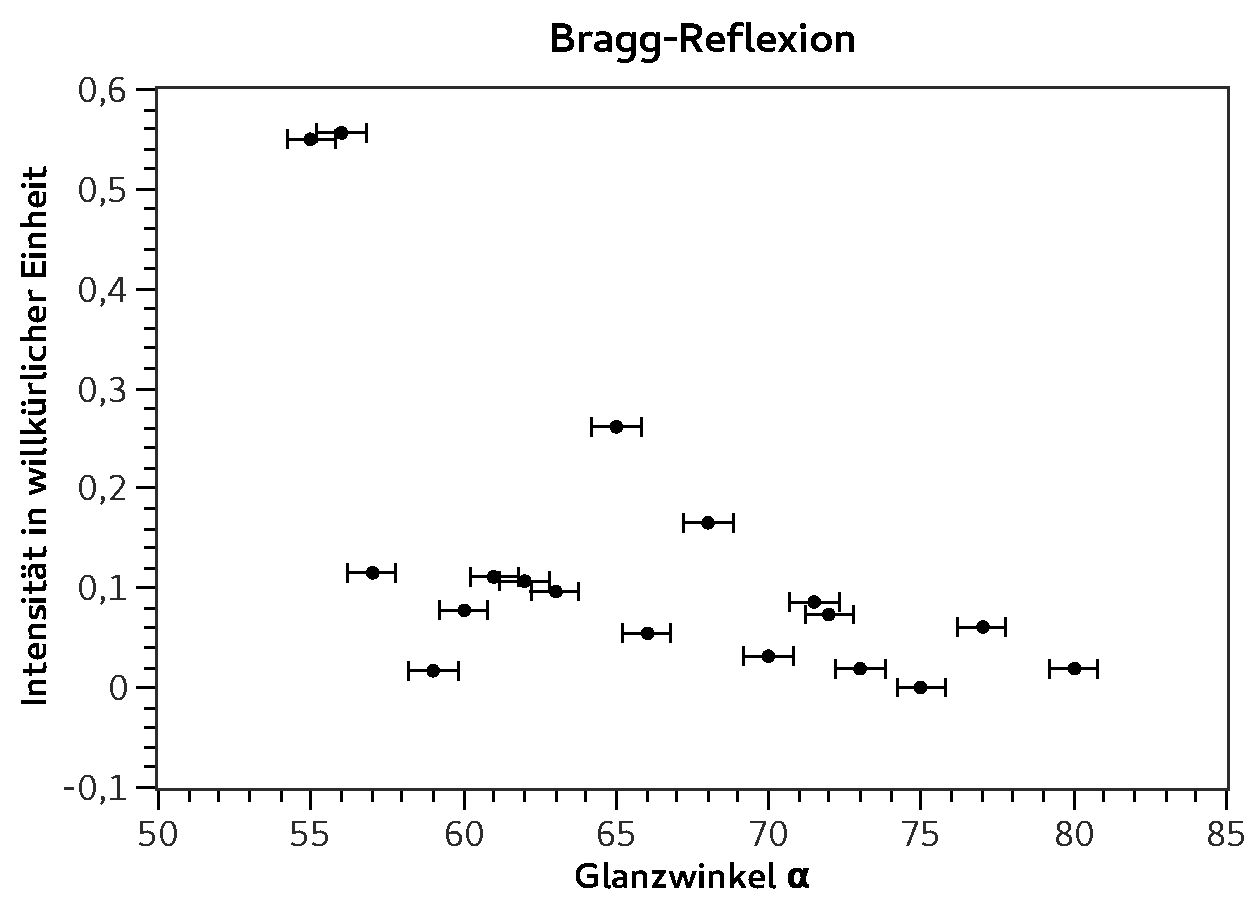
\includegraphics[width=0.7\textwidth]{fig_bragg}
		\centering
		\caption{Gemessene Intensität der Reflexionsstrahlung im Ausfallswinkel $2\alpha$ bei einem Einfallswinkel von $\alpha$.}
		\label{fig_bragg}
		\centering
	\end{figure}
	\subsection{Diskussion}
	%TODO Bezug/Nutzen oder sonst was
	%TODO auch hier die Hypothese wiederholen
	%TODO keine Messwerte hier, nach manchen Menschen, zumindest "direkt" erstellte Diagramme net hier, auch wenn Lesbarkeit-bla

	%TODO fraglich ob 1/r^2 von Maximums den Quellfleck genau bestimmt, da das mehr fürs Nahfelddd gilt und der Sender nicht bei nem Abstand von 0, Unendlich WElleintensität pumpen kann.
	
	\section{Schlussfolgerung}
	%TODO Rückgriff auf Hypothese und drittes Nennen dieser
	
	%TODO Quellen zitieren, Websiten mit Zugriffsdatum
	%TODO Verweise auf das Laborbuch (sind erlaubt)
	%TODO Tabelle + Bilder mit Beschriftung
	%\printbibliography
\end{document}
